

In this section we build up to our 
main contribution, the Composited Spatially Transformed Variational Auto-encoder model in three pieces. 
We first review the (vanilla) Variational Auto-encoder model, a deep generative model that
was recently proposed  in~\cite{Kingma2014}.  We next show how to factor pose from content
by introducing Spatially Transformed Variational Auto-encoders (ST-VAE).  Compositing multiple image layers generated
by ST-VAE modules 
finally allows us to create our desired CST-VAE model.



\subsection{{\bf VAE} Model: Variational Auto-encoder}\label{sec:vae}

Throughout this section, we are concerned with the following latent variable model.
Given a collection of i.i.d. samples $\{x_i\}_{i=1}^N$, we assume that each sample $x$
is generated by first drawing a variable $z$ independently from a prior distribution $P_\theta(z)$
then drawing $x$ conditioned on $z$ from $P_\theta(x|z)$.  %Thus we assume $P_\theta(x) = \int_z P_\theta(x | z) P_\theta(z) dz$.

The variable $z$ is assumed to be unobservable 
and we are thus interested in two coupled problems:
(inference) inferring $z$ given an observation $x$ and model parameters $\theta$, and 
(learning) estimating the model parameters $\theta$ given a collection of $x$.

If we want to model complicated data (e.g., images), however, we need to allow for rich conditional distributions
$P_\theta(x|z)$, which leads to complicated posteriors $P_\theta(z|x)$ making inference and learning intractable.

In the variational auto-encoding setting, we assumed a fixed form for the posterior distribution $Q_\phi(z|x)$ and optimize
the parameter $\phi$ to make $Q$ a good approximation to the posterior.  In contrast to typical mean-field approximations for latent variable models,
this optimization is not done per-instance    
Specifically we optimize the following 
which is a lower bound on the observed data log-likelihood:
\begin{equation}\label{eqn:vae_objective}
\mathcal{L}(\theta, \phi; x_i)
\end{equation}

The posterior parameterization $Q$ is sometimes called a \emph{recognition model} or a probabilistic \emph{encoder} (since we can
think of the latent variable $z$ as being a code
When $Q_\phi(z|x)$ is gaussian of the form () and  the mu and sigma and $P_\theta(x|z)$ can be written as
compositions of differentiable functions (i.e. neural networks), then the stochastic variational lower bound can be 
written in an end-to-end
differentiable way via the so-called \emph{reparameterization trick} introduced in ~\cite{Kingma2014}.
Furthermore, the objective can be interpreted as a reconstruction cost plus regularization term on the middle layer
of a neural network, which is why we think of these models as autoencoders.

%Both of the models that we discuss later in this section (i.e., ST-VAE and CST-VAE) fall under the category of variational auto-encoders,
%which was 



\subsection{{\bf ST-VAE} Model: Spatially Transformed Variational Autoencoder}\label{sec:stvae}


\begin{figure}[t]
\begin{center}
\subfigure[]{
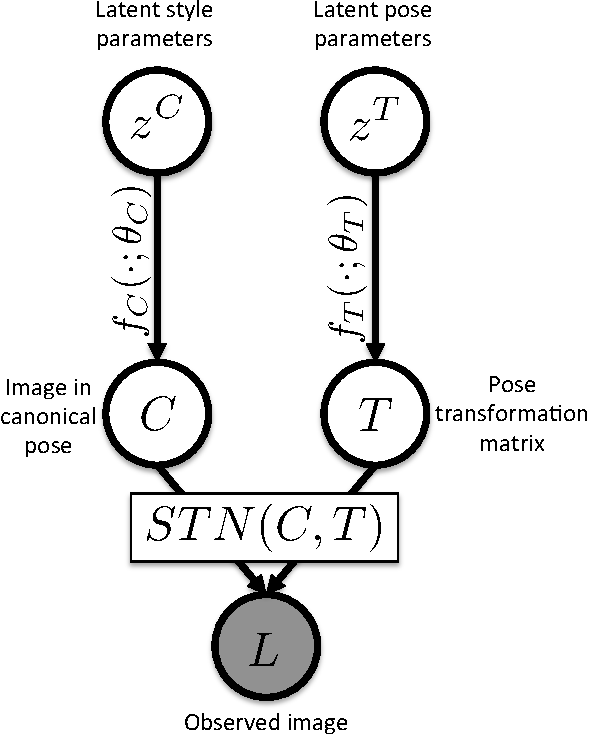
\includegraphics[width=0.2\linewidth]{figs/stvae_gen.pdf}
\label{fig:stvae_decoder}
}\qquad
\subfigure[]{
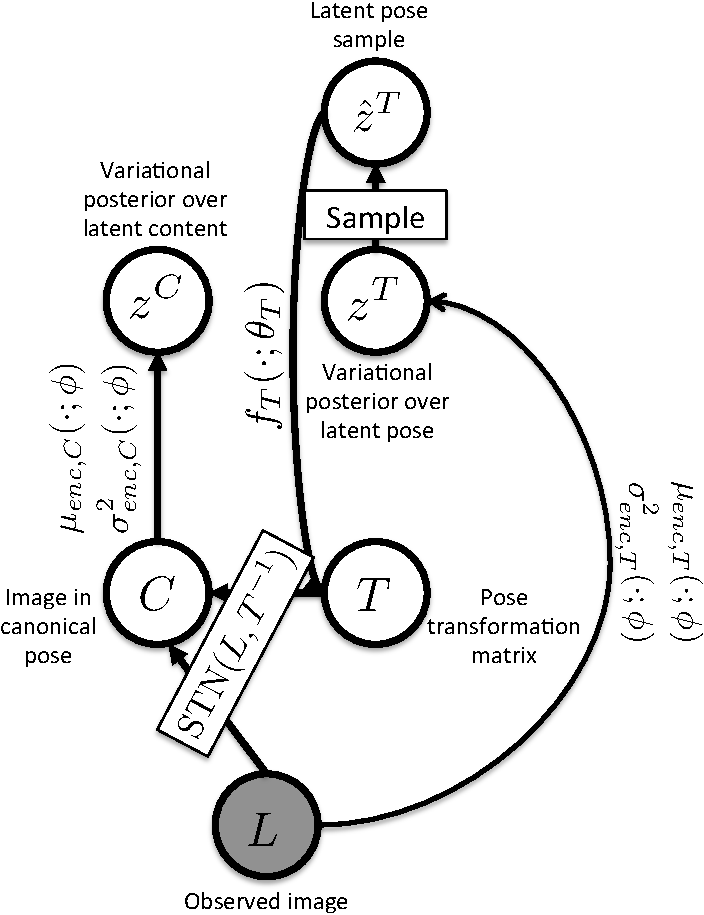
\includegraphics[width=0.20\linewidth]{figs/stvae_rec.pdf}
\label{fig:stvae_encoder}
}\qquad
\subfigure[]{
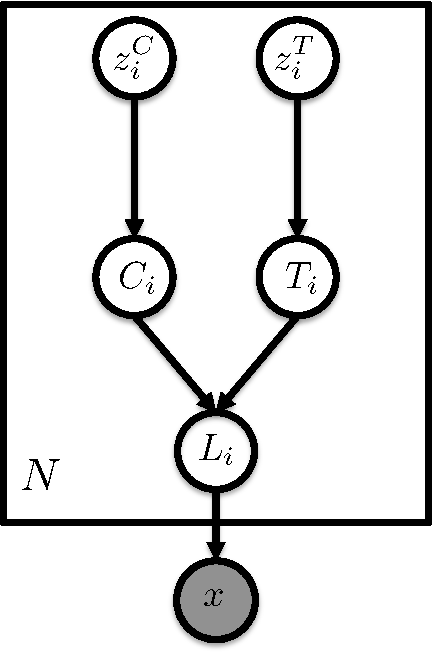
\includegraphics[width=0.2\linewidth]{figs/compositestvae_graphicalmodel.pdf}
\label{fig:compositestvae_gm}
}
\end{center}
 \caption{\subref{fig:stvae_decoder} ST-VAE Generative model, $P(x^\theta | z,\phi)$ (Decoder); \subref{fig:stvae_encoder} ST-VAE Recognition model $Q(z,\phi |x^\theta) = Q(z | \phi,x^\theta)\cdot Q(\phi|x^\theta)$ (Encoder); \subref{fig:compositestvae_gm} CST-VAE Generative model (plate notation).  }
 
\label{fig:stvaemodel}
\end{figure}


The Spatially transformed variational auto-encoder is a generative model of images of where pose and content are explicitly separated.  
We will think specifically of the case where the image is of a single object with a well-defined pose --- though there is nothing about the model
that prevents it from being applied to arbitrary images.
Specifically we assume that an image of an object is parameterized by a latent vector of content parameters 
$z$ as well as a latent vector of pose parameters $\phi$,
where both $z$ and $\phi$ are drawn independently from distributions $P(z)$ and $P(\phi)$.  
We then assume that the final observed image is generated by (1) first generating an image $x$ of the object in ``canonical pose'' conditioned on $z$,
then (2) generating reified transformation parameters $\theta$ conditioned on $\phi$, then (3) transforming the canonical image from the first step to form the 
final image $x^\theta$.  In our experiments $\theta$ is a vector of entries of a 2d affine transformation matrix, but more general transformations are also possible under our
framework.  
By explicitly allowing for  transformations of the image, we make modeling the content a much easier problem since the function $f(z)$ only needs to 
model the object in a particular canonical pose setting.

More specifically, the generative ST-VAE model is as follows:
\begin{align*}
z,\phi &\sim \mathcal{N}(0, I), \\
x &= f_z (z), \\
\theta &= f_\phi (\phi), \\
x^\theta &= \mbox{STM}(x, \theta),
\end{align*}
where $f_z$ and $f_\phi$ are neural networks (MLPs or convolutional networks) which we
refer to as  the content and pose decoders respectively, following the VAE terminology.
The function $\mbox{STM}(x, \theta)$ is a \emph{Spatial Transformer Network} module, recently introduced by Jaderberg et al~\cite{jaderberg2015spatial},
which resamples an image $x$ onto a regular grid which has been transformed by $\theta$ in a fully differentiable manner.
See Figure~\ref{fig:stvae_decoder} for a graphical representation of the ST-VAE generative distribution.

The next question is how to parameterize the recognition network.  Na\"{i}vely, one could 
simply use an ordinary MLP to parameterize distribution $Q(z, \phi | x)$, but ideally we would take advantage of the same
 insight that we used for the generative model: that it is advantageous to relate content to images in a canonical pose instead
 of conflating the two.  To this end, we propose the ST-VAE recognition model (see Figure~\ref{fig:stvae_encoder}). 
Conceptually the ST-VAE recognition model breaks the prediction of $z$ and $\phi$ into two stages.  Given the observed image $x^\theta$,
we first predict the latent representation of the pose, $\phi$.  Then we use $\phi$ to ``undo'' the transformation of the generative process
by using the Spatial Transformer Network again but this time using the inverse transformation of the predicted pose.  This result, which can be
thought as a prediction of the image in a canonical pose is finally used to predict latent style parameters.

More precisely, we assume that pose and content are independent in the variational posterior with
$Q(z, \phi | x) = Q(\phi |x)\cdot Q(z |\hat{\phi}, x)$ where both factors are normal distributions.  
To obtain a draw $(\hat{z}, \hat{\phi})$ from this posterior, we use the following procedure:

\begin{align*}
\hat{\phi} &\sim Q(\phi|x) = \mathcal{N}(\mu_\phi(x), \mbox{diag}(\sigma_\phi^2(x))), \\
\hat{\theta} &= f_\phi(\hat{\phi}), \\
\hat{x} &= \mbox{STM}(x^\theta, \theta^{-1}), \\
\hat{z} &\sim \mathcal{N}(\mu_z(\hat{x}), \mbox{diag}(\sigma_z^2(\hat{x}))).
\end{align*}

To train a model, we
optimize a similar lower bound as in Equation~\ref{eqn:vae_objective} with respect to parameters of the pose and content encoders/decoders:
\[
a+b
\]
As with the VAE, the ST-VAE objective is fully differentiable end-to-end.

For binary images, it is common to have a sigmoid at the end of the VAE decoder.
However we have found that it is often more numerically stable in these situations to first apple the spatial transformation, then
to apply the sigmoid after the transformation.

%We first predict a posterior over latent pose
%$Q(\phi |x^\theta)$.  We then use a sample $\phi\sim Q(\phi | x^\theta)$ and compute transformation parameters $\theta=f_\phi(\phi)$.  We then use
%the Spatial Transformer network again to transform the observed image $x^\theta$, this time using the inverse transformation $\theta^{-1}
%transform the observed image $x^\theta$ 
% which factors
% $Q(z, \phi | x) = Q(z | \phi, x)\cdot Q(\phi|x)$
  
 
 
 


\subsection{{\bf CST-VAE} Model: Composited Spatially Transformed Variational Autoencoder}\label{sec:cstvae}


\begin{figure}[t]
\begin{center}
\subfigure[]{
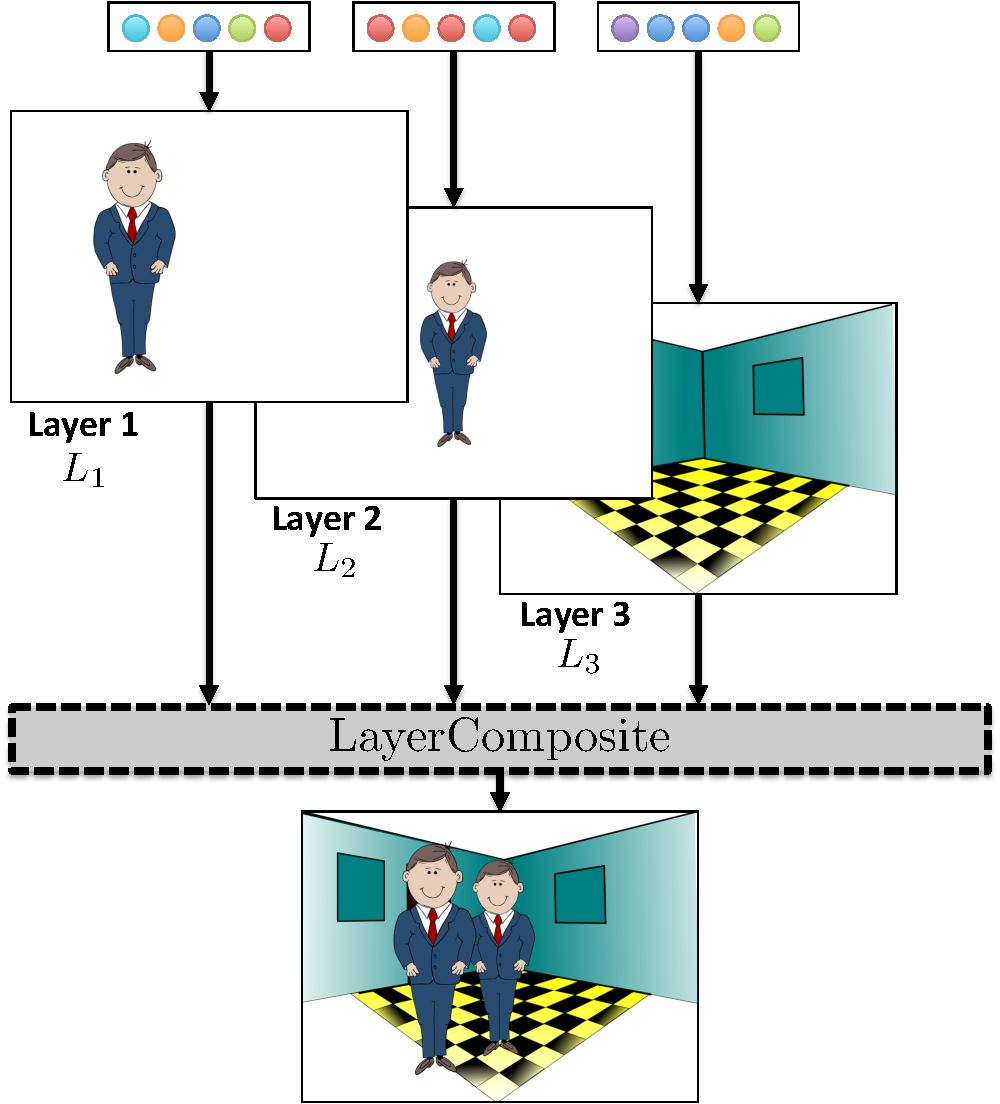
\includegraphics[width=0.30\linewidth]{figs/cartoon.pdf}
\label{fig:cartoon}
}\qquad
\subfigure[]{
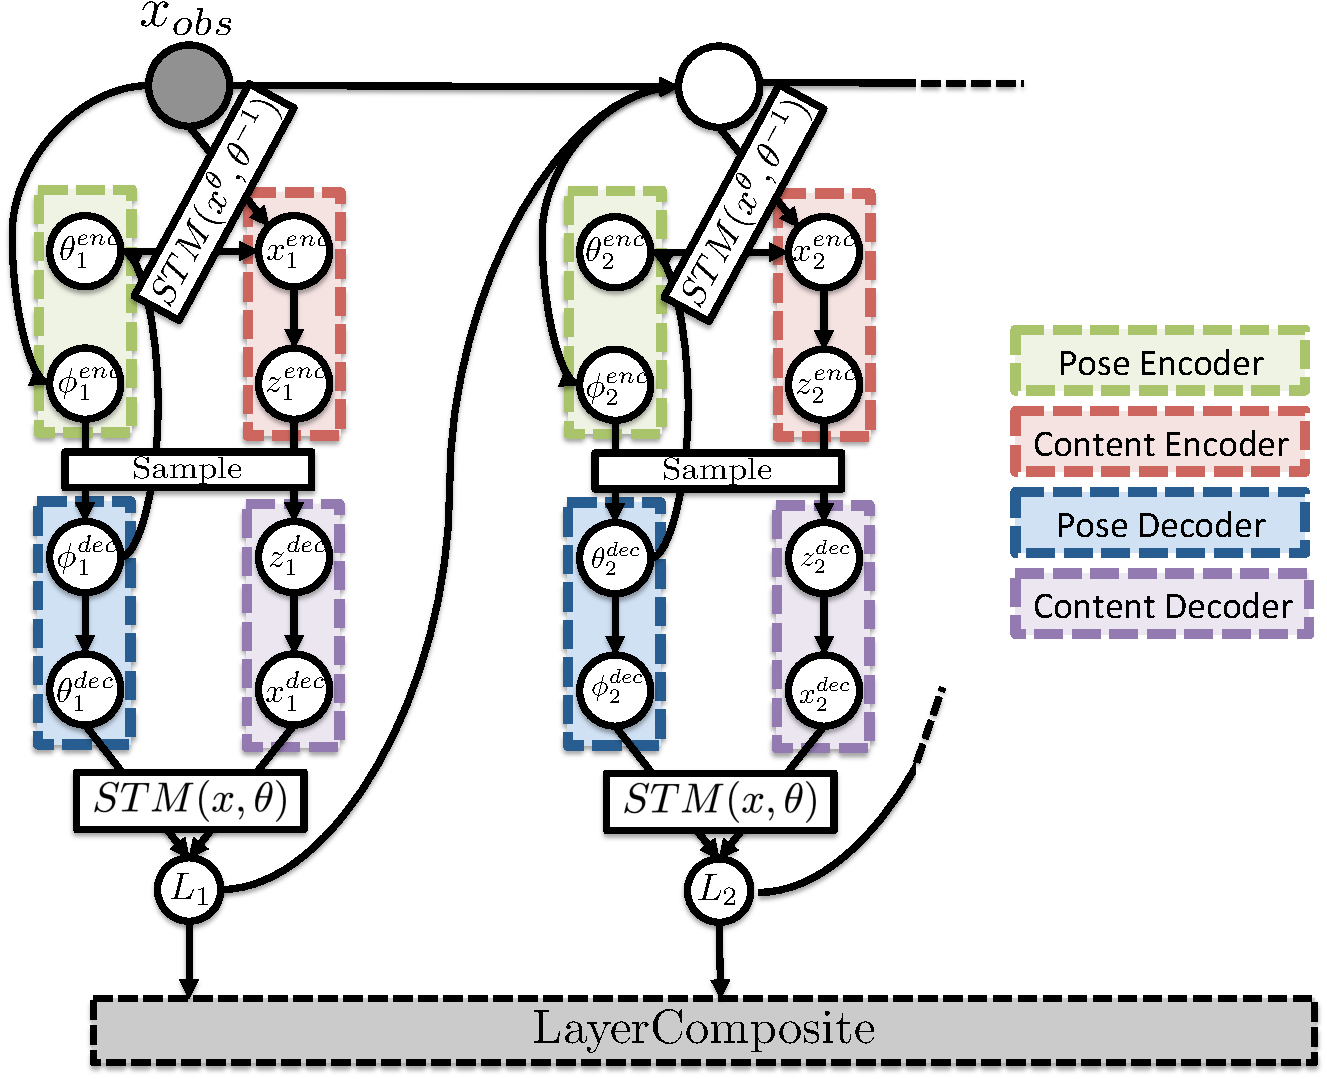
\includegraphics[width=0.55\linewidth]{figs/compositestvae.pdf}
\label{fig:cstvae}
}
\end{center}
 \caption{
 \subref{fig:cartoon} Simplified cartoon illustration of the CST-VAE layer compositing process; 
 \subref{fig:cstvae} The CST-VAE network unrolled for two layers.
 }
\label{fig:stvaemodel}
\end{figure}

Intuitively the ST-VAE model should work well in factoring pose from content for images of single objects.
However images generally contain multiple objects of different types with different poses --- we now present
the Composited Spatially Transformed Variational Auto-encoder  (CST-VAE) model, which is able to factor
the appearance of an image into the appearance of the different layers
that create an image.  
%The CST-VAE model thus makes it possible to combine generative models for images
%of single objects to obtain a generative model of  images of multiple objects.  
Among other things, the CST-VAE model allows us to tease
apart the component layers (or objects) that make up an image and reason about occlusion.
Furthermore, as we show in experiments, it can be trained in a fully unsupervised fashion using ordinary stochastic
gradient descent methods.  %However we can also add labels or use semi supervised methods a la asdfasdf

In the CST-VAE model, we  assume that images are generated by first independently generating a sequence of layers 
 via the ST-VAE model, then compositing layers from front to back to form a final observed image.  See Figure~\ref{fig:compositestvae_gm} for
 a graphical model depiction of the CST-VAE generative model and Figure~\ref{fig:cartoon}
 for a simplified cartoon illustration of the same process.  We assume that each layer is generated using the same ST-VAE model
 (i.e. parameters are shared across image layers). To composite these layers,  we use  the
classic \emph{over operator} from computer graphics~\citep{porter1984compositing}.
In the two-layer setting
with only foreground and background layers, this over operator reduces to a simple $\alpha$-weighted
convex combination of foreground and background pixels, but it extends in a natural (and differentiable)
way to handle multiple layers. % associativity of the over operator


As with the ST-VAE model, a critical design choice is how to parameterize the recognition model (encoder) --- in particular we would like to 
avoid learning a model that must make a ``straight-shot'' joint prediction of all objects and their poses in an image.
Instead our approach is to perform inference over a single layer at a time from front to back, each time removing the contribution of a layer
from consideration until the last layer has been explained.
More specifically, to perform inference for a single layer $i$, we use the ST-VAE module to generate a sample of the layer $L_i$.
We then compute $\mbox{ReLU}(x-L_i)$. \Jon{fix notation here!} which can be interpreted as the residual image --- the part of the image that is yet to be explained
by some layer.
Assuming that observed and predicted pixel values are between 0 and 1, $x-L_i$ can be negative, which breaks interpretability of the layers --- the
ReLU transfer function serves to ensure that the residual image can always itself be interpreted as an image.
Figure~\ref{fig:cstvae} unrolls the entire network for two layers.

% Can we easily interpret what we're doing as a legitimate recognition model?

Write out objective function.













